
\documentclass{article}
\usepackage{a4wide}
\usepackage[utf8]{inputenc}
\usepackage{amsmath}
\usepackage{mathtools}
\usepackage{amssymb}
\usepackage[english]{babel}
\usepackage{mdframed}
\usepackage{systeme,}
\usepackage{lipsum}
\usepackage{relsize}
\usepackage{caption}
\usepackage{tikz}
\usepackage{tikz-3dplot}
\usepackage{pgfplots}
\usepackage{harpoon}%
\usepackage{graphicx}
\usepackage{wrapfig}
\usepackage{subcaption}
\usepackage{authblk}
\usepackage{float}
\usepackage{listings}
\usepackage{xcolor}
\usepackage{amsmath}
\usepackage{chngcntr}
\usepackage{amsthm}
\usepackage{comment}
\usepackage{commath}
\usepackage{hyperref}%Might remove, adds link to each reference
\usepackage{url}
\newcommand{\w}{\omega}
\newcommand{\curl}[1]{\mathbf{\nabla}\times \mathbf{#1}}
\newcommand{\grad}{\mathbf{\nabla}}
\newcommand{\dive}[1]{\mathbf{\nabla}\cdot \mathbf{#1}}
%\newcommand{\crr}{\mathfrak{r}}
\usepackage{calligra}

\DeclareMathAlphabet{\mathcalligra}{T1}{calligra}{m}{n}
\DeclareFontShape{T1}{calligra}{m}{n}{<->s*[2.2]callig15}{}
\newcommand{\crr}{\mathcalligra{r}\,}
\newcommand{\boldscriptr}{\pmb{\mathcalligra{r}}\,}
\newcommand{\res}[2]{\text{Res}(#1,#2)}

\title{Handin 7}
\author{Author : Andreas Evensen}
\date{Date: \today}
\definecolor{codegreen}{rgb}{0,0.6,0}
\definecolor{codegray}{rgb}{0.5,0.5,0.5}
\definecolor{codepurple}{rgb}{0.58,0,0.82}
\definecolor{backcolour}{rgb}{0.95,0.95,0.92}

\lstdefinestyle{mystyle}{
    backgroundcolor=\color{backcolour},   
    commentstyle=\color{codegreen},
    keywordstyle=\color{magenta},
    numberstyle=\tiny\color{codegray},
    stringstyle=\color{codepurple},
    basicstyle=\ttfamily\footnotesize,
    breakatwhitespace=false,         
    breaklines=true,                 
    captionpos=b,                    
    keepspaces=true,                 
    numbers=left,                    
    numbersep=5pt,                  
    showspaces=false,                
    showstringspaces=false,
    showtabs=false,                  
    tabsize=2
}

\lstset{style=mystyle}

\begin{document}

\maketitle

\section*{Warmup}

\subsection*{a)}
\begin{align*}
    \beta(p, q) = \frac{\Gamma(p)\Gamma(q)}{\Gamma(p+q)}
\end{align*}
Compute $\beta(4,3)$
\begin{align*}
    \beta(4, 3) &= \frac{\Gamma(4)\Gamma(3)}{\Gamma(7)}\\
    &=\frac{3!\cdot2!}{6!} = \frac{2}{4\cdot 5 \cdot 6} = \frac{1}{60}
\end{align*}
\subsection*{b)}
Calculate the general solution of $\ln(1+i)$. One begin by stating $1 + i = z$, and thus $z$ can be expressed in euler form.
\begin{align}
    \ln(1 + i) &=\ln(z)\nonumber\\
    &=\ln\left(\sqrt{2}\exp\left[i\arctan(1)\right]\right)\nonumber\\
    &=\ln\left(\sqrt{2}\exp\left[i\frac{\pi}{4}\right]\right)\nonumber\\
    &= \sqrt{2}\Big(i\frac{\pi}{4} + n2\pi i\Big) ; \quad n \in\mathbb{Z}\label{eq: task1b}
\end{align}

\section*{Complex integral with branch-cut}

\subsection*{a)}
The function $\ln(z)$ is not contionous in the complex plane, due to eq \eqref{eq: task1b}, since $n$ is an integer; $\ln(z)$ does a phase-shift of $2\pi$ for every integer $n$.
Now suppose a function $f(z) = z^\alpha$ $\forall \alpha \in[0, \infty)$. One wish to find whether such a function is contionous:
\begin{align*}
    f(z) &= z^\alpha = \left(r\exp[i\theta]\right)^\alpha = r^\alpha\exp[i\theta\alpha]
\end{align*}The function $f(z) = z^\alpha$ is contionous for all $\alpha \in \mathbf{Z}^+$ but for every other value of $\alpha$ is is not contionous, and we get a branch-point.


\subsection*{b)}
\begin{align}
    I = \int_0^\infty \frac{dx}{x^\alpha(x + p)}\label{eq: task2b}
\end{align}
\subsubsection*{I}
To check whether the expression \eqref{eq: task2b} converges one firstly check the behaviour of the integrand as $x\rightarrow 0$ and $x\rightarrow \infty$.
\begin{align*}
    I =\int_0^\infty \frac{dx}{x^{\alpha + 1} + x^{\alpha}p}.
\end{align*}As the limit approches infinity, the integral converges for $\alpha>1$ but when the limit approaches zero, it diverges for all $\alpha\notin[0, 1)$.
Thus the integral converges for $\alpha\in[0, 1)$ and diverges for $\alpha\notin[0, 1)$.

\subsubsection*{II}
Considered the contour from figure (11.26) in Arfken, one computes the following integral:
\begin{align*}
    \oint_C \frac{dz}{z^\alpha(z + p)} = 0.
\end{align*}One computes the find the singularities of the integrand:
\begin{align*}
    z^\alpha(z + p) &= 0\\
    \implies z &= 0, \quad z = -p
\end{align*}
Computing the residues at the singularties, at $z = -p$ which is a single pole, one finds the following: 
\begin{align*}
    \res{f}{-p}\lim_{z\to -p} (z+p)\frac{1}{z^\alpha(z + p)} = \frac{1}{(-p)^{\alpha}} = \frac{1}{(-1)^\alpha\cdot(p)^\alpha}\\
\end{align*}
Given the countour, we avoid the point $z = 0$, and thus the residue at $z = 0$ is zero. Using this one computes the following:
\begin{align*}
    \oint_C \frac{dz}{z^\alpha(z + p)} &= \int_0^\infty \frac{dr}{r^\alpha(r + p)} + \int_{\infty}^0\frac{e^{-2\pi i \alpha}dr}{r^\alpha(r + p)} \\
    &= \int_0^\infty \frac{dr}{r^\alpha(r + p)} - e^{-2\pi i \alpha}\int_{0}^\infty\frac{dr}{r^\alpha(r + p)} \\
    &= (1-e^{-2\pi i \alpha})I = 2\pi i\sum_i \res{f}{z_i}\\
    \implies I&= \frac{2\pi i\sum_i\res{f}{z_i}}{1-e^{-2\pi i \alpha}}\\
    &=2\pi\frac{1}{p^{\alpha}}\left(\frac{1}{\frac{\sin(\pi \cdot\alpha)}{2\pi}}\right) = \frac{\csc(\pi \alpha)}{p^\alpha}\\
    \text{Reflection formula: }&= \frac{\Gamma(\alpha)\Gamma(1-\alpha)}{p^\alpha}.
\end{align*}This is the identity one wished to show.


\subsection*{c)}
\begin{align*}
    J = \int_0^\infty\frac{\ln(x)dx}{a^2 + x^2}
\end{align*}
\subsubsection*{I}
The complex logarithm for $\ln(x)$ for $x\in(-\infty, 0)$ is defined as:
\begin{align*}
    \ln(x) = \ln(|x|) + i\pi.
\end{align*}In other words, there exists a phase-shift, which results in result to lie in the complex plane.

\subsubsection*{II}
Firstly one defines the following:
\begin{align}
    \oint \frac{\ln(z)}{z^2 + a^2}dz.
\end{align}Secondly, one computes the singularities of the integrand:
\begin{align*}
    z_0 = 0\\
    z_{1,2} =\pm ai
\end{align*}The objective is not to define a contour which encloses one of the singularities but not both, and avoids the branch-cut. One defines the following contour:
\begin{figure}[H]
    \centering
    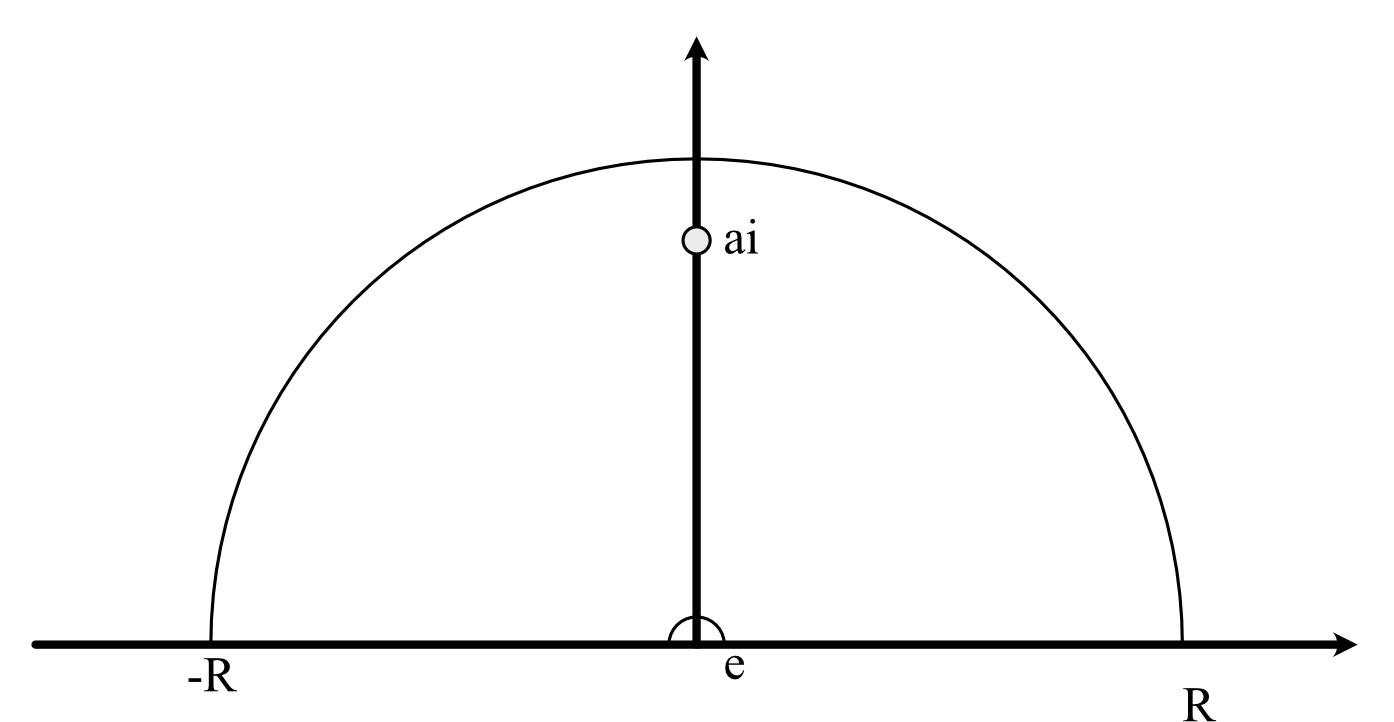
\includegraphics[scale = 0.5]{image.png}
    \caption{The contour $C$, but the right side of the branch-cut is not included.}
    \label{fig: 3cII}
\end{figure}\noindent Thus the closed contour integral becomes:
\begin{align*}
    \oint_C \frac{\ln(z)}{z^2 + a^2}dz &= \lim_{R\to\infty,\epsilon\to0}\int_\epsilon^R \frac{\ln(x)}{x^2 + a^2}dx + \int_{arc}f(z)dz + \int_{-R}^{-\epsilon}\frac{\ln(z)}{z^2 + a^2}dz\\
    &= \lim_{R\to\infty,\epsilon\to0}\int_\epsilon^R \frac{\ln(x)}{x^2 + a^2}dx - \int_{-\epsilon}^{-R}\frac{\ln(r e^{i\theta})}{r^2 + a^2}dr\\
    &= \lim_{R\to\infty,\epsilon\to0}\int_\epsilon^R \frac{\ln(x)}{x^2 + a^2}dx + \int_{\epsilon}^{R}\frac{\ln(r e^{-i\theta})}{r^2 + a^2}dr\\
    &= \lim_{R\to\infty,\epsilon\to0}\int_\epsilon^R \frac{\ln(x)}{x^2 + a^2}dx + \int_{\epsilon}^{R}\frac{\ln(r)-i\theta}{z^2 + a^2}dr\\
    &= \lim_{R\to\infty,\epsilon\to0}\int_\epsilon^R \frac{\ln(x)}{x^2 + a^2}dx + \int_{\epsilon}^{R}\frac{\ln(r)}{r^2 + a^2}dr - \int_\epsilon^R \frac{i\theta}{z^2 + a^2}\\
    &= \lim_{\epsilon\to0}2\cdot I - \int_\epsilon^R\frac{i\theta}{z^2 + a^2}dz
\end{align*}In this instance, $\theta$ is a fixed value close to $\pi$
\begin{align*}
    \lim_{\epsilon\to0} \frac{i}{2}\oint\frac{\pi - \epsilon}{z^2 + a^2}dz =\lim_{\epsilon\to0} \frac{i(\pi - \epsilon)}{2}\left(2\pi i\frac{1}{2ai}\right) = \frac{i\pi^2}{2a}
\end{align*}Thus one has the following:
\begin{align*}
    \oint_c f(z)dz &= 2 I - \frac{i\pi^2}{2a} = \pi\frac{\ln(ai)}{a}\\
    \implies I &= \frac{1}{2}\left(\pi\frac{\ln(ai)}{a} + \frac{i\pi^2}{2a}\right)\\
    &= \frac{1}{2}\left(\pi\frac{\ln(a)}{a} - \frac{i\pi^2}{2a} + \frac{i\pi^2}{2a}\right)=\frac{\ln(a)\pi}{2a}
\end{align*}
\begin{comment}
Firstl
Defining the complex contour closed $(0,R)-(R, a)-(-R, a)-(-R, 0)$ when letting $R\rightarrow \infty$. We use the following:
$z=re^{i\theta}$, $dz = ire^{i\theta}d\theta$, which implies $d\theta = -i\cdot z^{-1}dz$.
\begin{align*}
    \oint f(z)dz &=\oint \frac{\ln(z)}{z^2 + a^2}dz = \oint \frac{\ln(re^{i\theta})}{z^2+a^2}\\
    &=\lim_{R\to\infty} \int_0 ^R + \int_{0}^a + \int_{R}^{-R} + \int_{a}^0 + \int_{-R}^0 \\
    &= \lim_{R\to\infty}\left[\int_0^R + \int_{-R}^0 + \int_{-R}^R + \int_0^{a}  - \int_{0}^{a}\right]\\
    &= \lim_{R\to\infty}\left[2\int_{-R}^R\right]\\
\end{align*}

\end{comment}


\section*{Integration of Bessel-functions}
\begin{align*}
    I_n = \int_0^\infty J_n(x)dx
\end{align*}
\subsection*{a)}
The Bessel-function of the first kind can be defined as:
\begin{align*}
    J_n(x) = \sum_{s =0}^\infty \frac{(-1)^s}{s!(s+n)!}\cdot\left(\frac{x}{2}\right)^{n+2s}.
\end{align*}To find the behavior as $x\to0$ and $x\to\infty$ one defines the following limits, (where $n$ is a fixed integer):
\begin{align*}
    \lim_{x\to x_i}J_n(x) &= \lim_{x\to x_i}\left[\sum_{s =0}^\infty \frac{(-1)^s}{s!(s+n)!}\cdot\left(\frac{x}{2}\right)^{n+2s}\right]\\
    &=\lim_{x\to x_i}\left[\sum_{s = 0}^\infty \frac{x^{n}}{(s+n)!}\cdot\underbrace{\frac{(-1)^2}{s!}\left(\frac{x}{2}\right)^{2s}}_{p_s(x)}\right]\\
    \implies& \lim_{x\to 0} J_n(x) = 0\\
    \implies& \lim_{x\to 0} J_0(x) = 1\\
    \implies& \lim_{x\to \infty} J_n(x) = 0
\end{align*}

\subsection*{b)}
Show $I_1 = -[J_0(x)]_{0}^\infty=1$. The special case for $n =0$ is given by:
\begin{align*}
    J_1(x)&=-J_0'(x)\\
    \implies \int_0^\infty J_1(x) &= -\int_0^\infty J_0'(x)dx\\
    I_1&=-\left[J_0(x)\right]_{x = 0}^\infty \\
    &= -(0 - 1) = 1
\end{align*}

\subsection*{c)}
One wishes to show$I_{n-1}=I_{n+1}$; in order to accomplish this, one defines the following integral: $Q = I_{n+1}-I_{n-1}$. Under the assumption that $Q$ is non-zero, we do the following computation:
\begin{align*}
    Q &= I_{n+1}-I_{n-1} = \int_0^\infty J_{n+1}(x) - J_{n-1}(x)dx\\
    &=\int_0^\infty dx\left[J_{n+1}(x) - J_{n-1}(x)\right]\\
    &=\int_0^\infty dx \left(2\cdot J_n'(x)\right)\\
    &=2\Big[J_n(x)\Big]_{x = 0}^\infty = 0.
\end{align*}
We've disproven the previous assumption, and thus $I_{n-1} = I_{n+1}$.

\subsection*{d)}
Compute $I_0$;
\begin{align*}
    I_0 &= \int_0^{\infty}J_0(x)dx\\
    &=\mathbf{R}\frac{1}{2\pi}\int_0^\infty dx\left(\int_0^{2\pi} d\theta\left(\exp\left[ix\cos(\theta)\right]\right)\right)\\
    \text{Fubinis theorem :}&=\mathbf{R}\frac{1}{2\pi}\int_0^{2\pi} d\theta\left(\int_0^{\infty} dx\left(\exp\left[ix\cos(\theta)\right]\right)\right)\\
    &= \mathbf{R}\frac{1}{2\pi}\int_0^{2\pi} d\theta\left[\left(\frac{\exp\left[ix\cos(\theta)\right]}{i\cos\theta}\right)\right]_{x = 0}^\infty\\
    &=\frac{1}{2\pi}\Bigg[\theta\Bigg]_{\theta = 0}^{2\pi} = 1
\end{align*}

\end{document}
    